Intraoperative X-Ray is essential during some surgeries, such as
percutaneous coronary intervention. The 2D X-Ray images not only lose
a significant amount of 3D information of the coronary arteries, but
also suffer from the viewing angle dependence, magnification factor,
overlapping and the blurring between vessels, backgrounds and other
tissues and organs.

Great efforts have been done on 3D reconstruction of coronary arteries
to overcome the shortcomings of 2D images. But there are also some
problems existing in current methods. First, the absence of image
enhancement procedures may lead to disappearance of some tiny details
because of the low contrast and blurring of angiograms. Second, the
vessel skeleton extraction methods are not accurate and may acquire
discontinuous or unsmooth results. Third, accurate reconstructions
need five or more views of angiograms with exact angle requirements,
which is hard to operate for clinical use. Fourth, current 3D
reconstruction methods mostly rely on the registrations between image
pairs, which are hard to add constrain conditions such as consistency
and continuity.

To overcome these shortcomings, we present an efficient vessel
reconstruction system from multiple X-Ray views. The pipeline is shown
in Figure \ref{fig:procedure}. First, we apply the multi-scale retinex
method to enhance the contrast of the angiogram. Second, we implement
a CUDA edition of Hessian matrix based vessel filter with hysteresis
thresholding to get the preprocessing results. Third, we perform the
fast-marching method using second order derivatives and cross neighbor
templates to extract the accurate centerline of the
vascular-structure. Finally, 3D reconstruction with local constraints
and space consistencies is formulated as an energy minimization
problem and solved using belief propagation. All these lead to a fast
reconstruction result of the data and promise accuracy and efficiency
which can give the doctor a good sense of coronary artery 3D space
structures. The contributions of the paper are:

(1) We combine the MSR enhanced images which are mostly over extracted
with line segments tracking methods to obtain more detailed vessels
from blurry angiograms.

(2) We divide the spaces between the X-Ray iso-center and the detector
into slices in which we sample the 3D space points and project them to
the image space considering consistency and continuity with their
neighbors, overcoming the lack of constraints for typical
registrations.

(3) We formulate the 3D reconstruction as a global energy
optimization problem and solve it by using belief propagation.


\begin{figure*}
  \centering
  % Requires \usepackage{graphicx}
  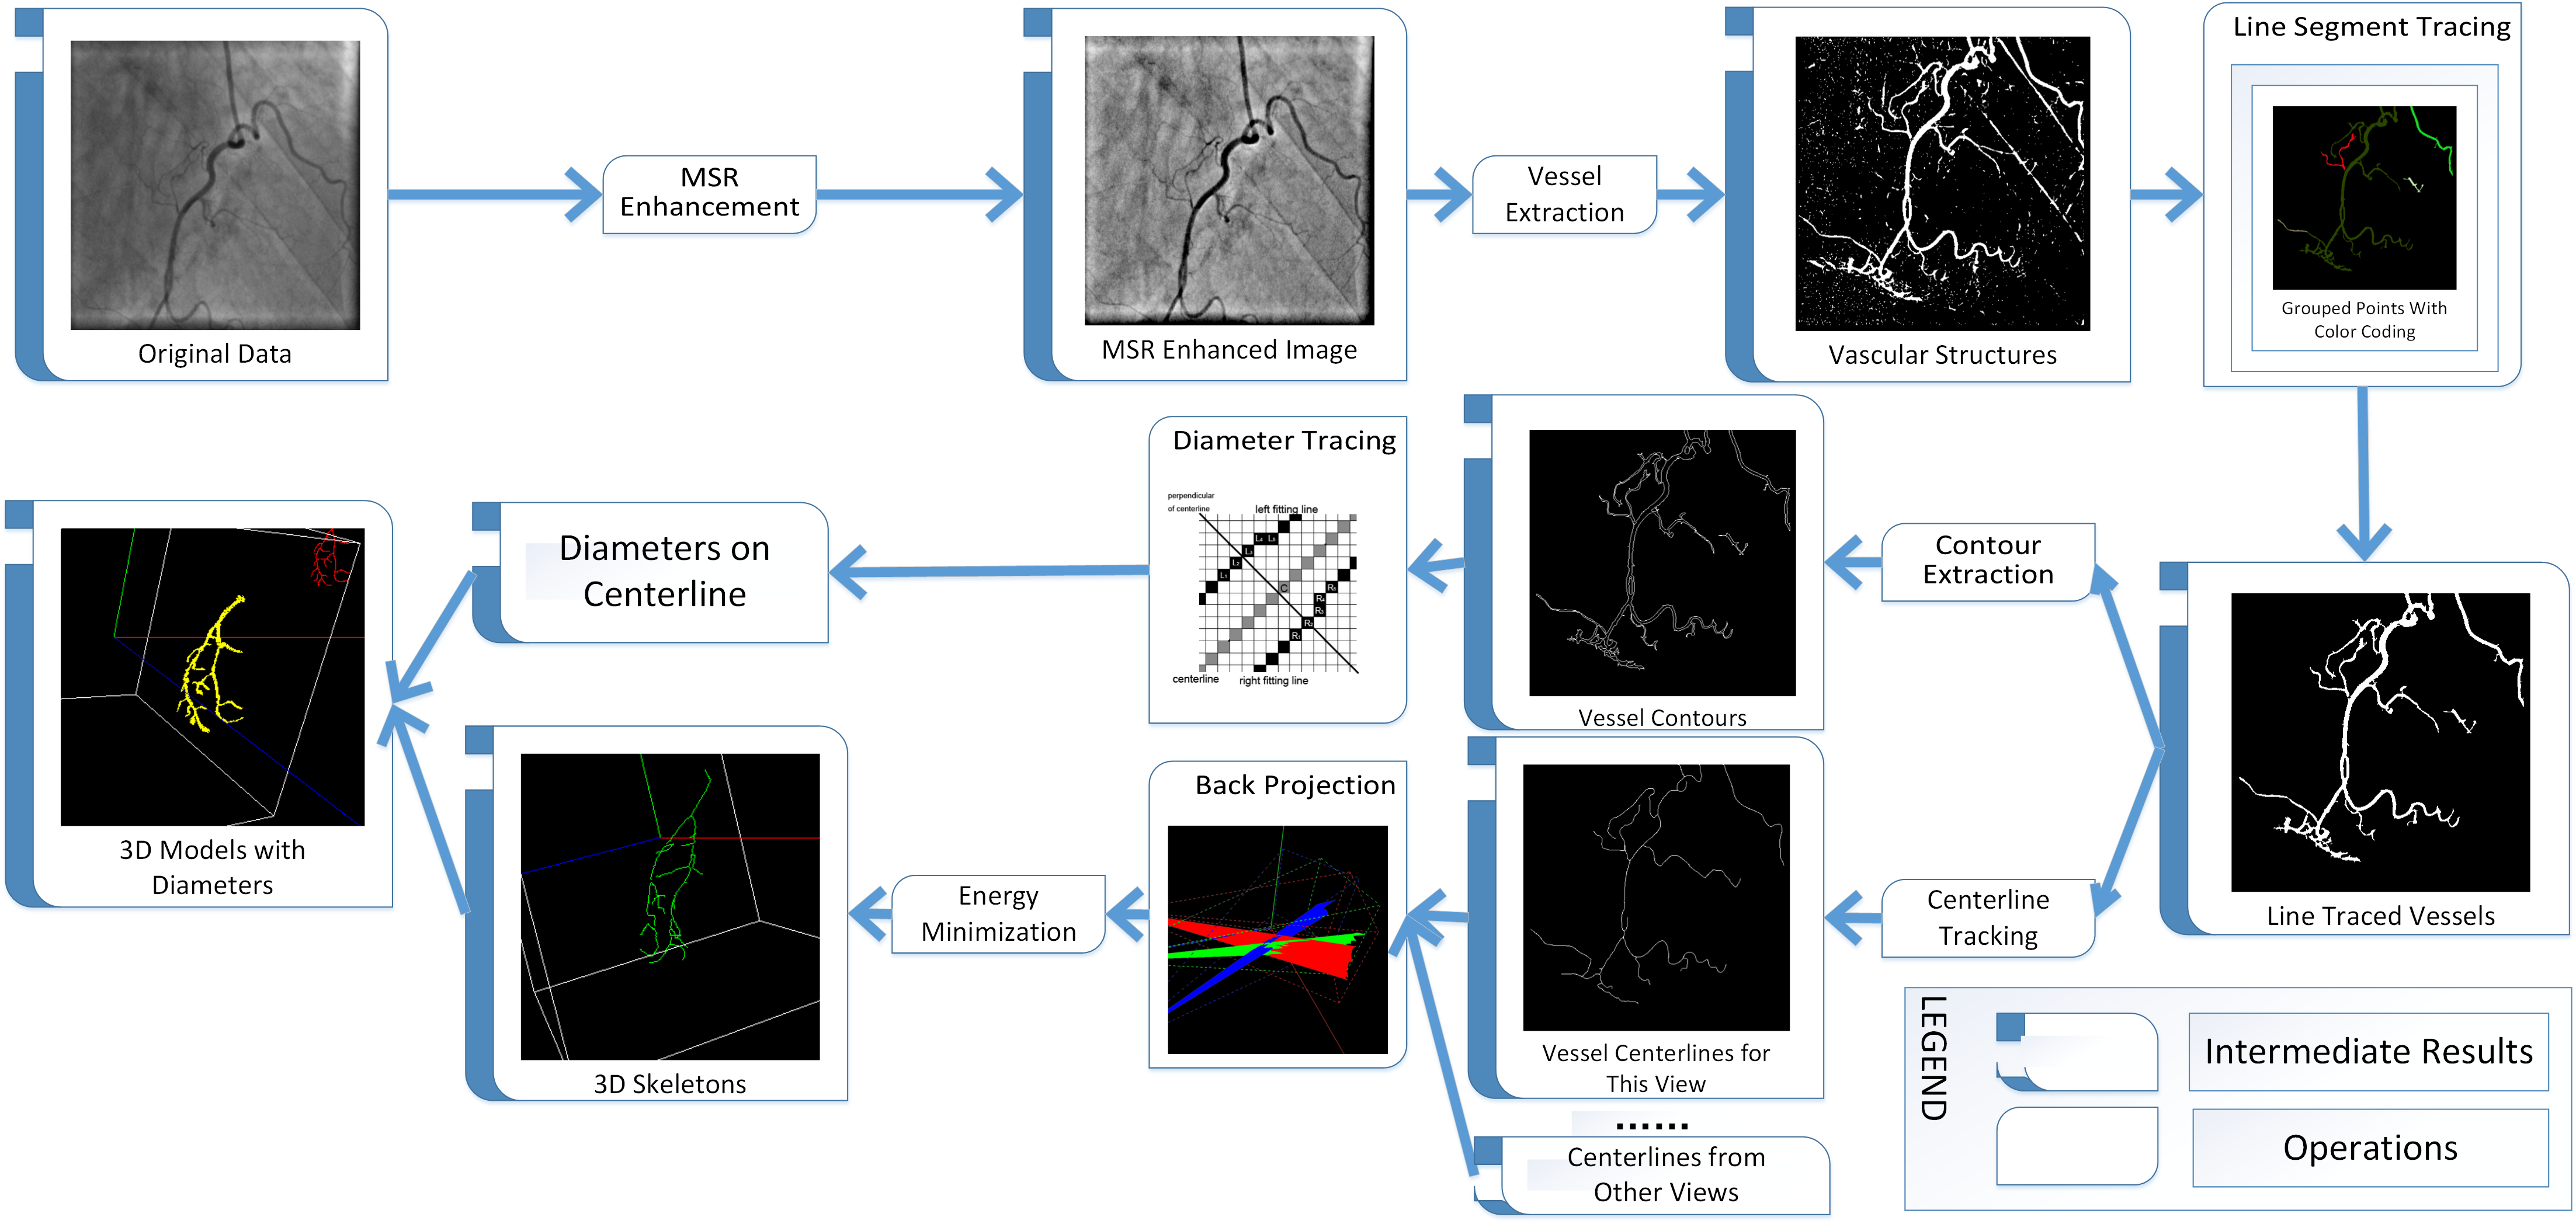
\includegraphics[width=6.0in]{procedure.png}\\
  \caption{Work Pipelines}\label{fig:procedure}
\end{figure*}
